\chapter{Letters}

\section*{{\normalsize Letter from Terry Riley, Paris, to Henry Flynt, Cambridge, Mass., \\ dated 11/8/62}}

One day a little boy got up and looked at his toys, appraised them and 
decided they were of no value to him so he did them in. Seeing that others 
were blindly and blissfully enjoying theirs he offered them a long and 
\enquote{radical new theory} of \enquote{pure recreation} for their enjoyment but before he 
let them in for this highly secret and \enquote{revolutionary theory} they should 
follow his example and partake of a little 20th C. iconoclasm. From those 
that balked he removed the label \enquote{avant-garde} and attached the label 
\enquote{traditionalist} or if they were already labeled \enquote{traditionalist} he added one 
more star. If they accepted they got a \enquote{hip} rating with gold cluster and if 
they comprehended the worth of his theory well enough to destroy their 
own art they would be awarded assignments to destroy those works whose 
designers were no longer around to speak out in their behalf. 

Now about this hip radical new theory of pure recreation.---Well---alor! its 
simply what people do anyway but don't realize it but it seems that what 
people \enquote{do anyway and don't realize it} will not be fully appreciated until 
\enquote{what people do in the name of art} is eliminated. If art can be relegated to 
obscurity, if some one can get John Coltrane to stop blowing, if someone 
can smash up all the old Art tatum records as well as all the existing pianos, 
if someone can get all that stuff out of those museums, If someone can only 
burn down all those concert halls, movie houses, small galleries as well as 
rooms in private houses that contain signs of art, If someone can do in all the 
cathedrals and monuments bridges etc, If someone can get rid of the sun, 
moon, stars, ocean, desert trees birds, bushes mountains, rivers, joy, sadness 
inspiration or any other natural phenomenon that reminds us of the ugly 
scourge art that has preoccupied and plagued man since he can remember 
then yes then at last Henry Flynt, sorry! 

{\centering 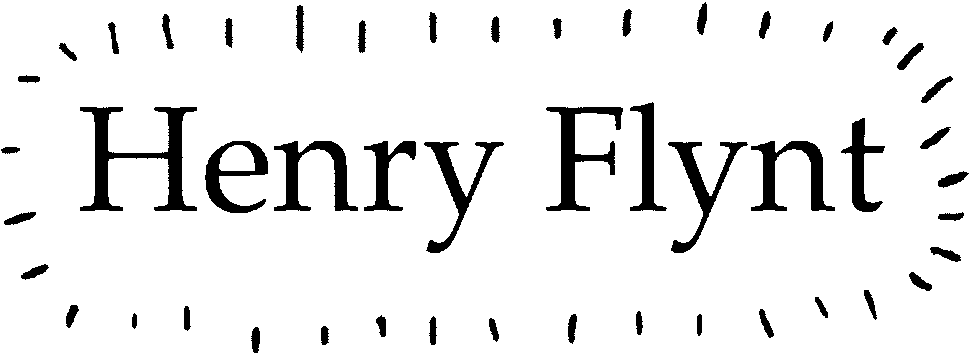
\includegraphics[width=3in]{terry_flynt_name} \par}

will show us how to really enjoy ourselves. Whooopeeee 
\vfill
\signoffnote{[Terry Riley's spelling etc. carefully preserved]}

\clearpage

\section*{{\normalsize Letter from Bob Morris to Henry Flynt, dated 8/13/62}}

\vfill 
\noindent
Dear Henry, \\
perhaps the desirability of certain kinds of experience in art is not 
important. The problem has been for some time one of ideas---those most 
admired are the ones with the biggest, most incisive ideas (e.g. Cage \& 
Duchamp). The mere exertion in the direction of finding \enquote{new} ideas has 
not shown too much more than that it has become established as a 
traditional method; not much fruit has appeared on this vine. Also it can't be 
avoided that this is an academic approach which presupposes a history to 
react against---what I mean here is the kind of continuity one is aware of 
when involved in this activity: it just seems academic (if the term can 
somehow be used without so much emotion attached to it). The difficulty 
with new ideas is that they are too hard to manufacture. Even the best have 
only had a few good ones. (I suppose none of this is very clear and I can't 
seem to get in the mood to do any more than put it down in an off-hand 
way---but what I mean by \enquote{new ideas} is not only what you might call
\enquote{Concept Art} but rather effecting changes in the structures of art forms 
more than any specific content or forms) Once one is committed to attempt 
these efforts---and tries it for a while---one becomes aware that if one wants 
\enquote{experience} one must repeat himself until other new things occur: a 
position difficult if not impossible to accept with large \enquote{idea} ambitions. So 
one remains idle, repeats things, or finds some form of concentration and 
duration outside the art---jazz, chess, whatever. I think that today art is a 
form of art history. 

I don't think entertainment solves the problem presented by avant gard art 
since entertainment has mostly to do with replacing that part of art which is 
now hard to get---i.e. experience. It seems to me that to be concerned with 
\enquote{just liked} things as you present it is to avoid such things as tradition in art 
(some body of stuff to react against---to be thought of as opponent or 
memory or however). As I said before, I for one am not so self-sufficient and 
when avoiding \enquote{given} structures, e.g. art, or even the most tedious and 
decorous forms of social intercourse, I am bored. If I need concentration, 
which I do, I can't think of anything on my own as good as chess. 

One accepts language, one accepts logic. 

\vfill

\signoff{Best regards,}
\signoff{Bob Morris}

\clearpage

\section*{}

{\raggedleft 
\parbox{2.5in}{
\textsc{From "Culture" to Veramusement} \\
Boston--New York \\
\textsc{Press Release:} for March--April, 1963 \par
}\vskip 1em}


Henry Flynt, Tony Conrad, and Jack Smith braved the cold to demonstrate 
against Serious Culture (and art) on Wednesday, February 27. They began at 
the Museum of Modern Art at 1:30 p.m., picketing with signs bearing the 
slogans 
\textsc{Demolish serious culture! / Destroy art!} ; 
\textsc{Demolish art museums! / No more art!} ;
\textsc{Demolish concert halls! / Demolish Lincoln Center!}
and handing out announcements of 
Flynt's lecture the next evening. Benjamin Patterson came up to give 
encouragement. There was much spontaneous interest among people around 
and in the Museum. At about 1:50, a corpulent, richly dressed Museum 
official came out and imperiously told the pickets that he was going to 
straighten them out, that the Museum had never been picketed, that it could 
not be picketed without its permission, that it owned the sidewalk, and that 
the pickets would have to go elsewhere. The picket who had obtained police 
permission for the demonstration was immediately dispatched to call the 
police about the matter, while the other two stood aside. It was found that 
the Museum official had not told the truth; and the picketing was resumed. 
People who care about the rights of pickets generally should recognize the 
viciousness of, and oppose, the notion that picketing can only be at the 
permission of the establishment being picketed. (As for previous picketing of 
the Museum, it is a matter of record.) Interest in the demonstration 
increased; people stopped to ask questions and talk. There was a much 
greater demand for announcements than could be supplied. Some people 
indicated their sympathy with the demonstrators. The demonstrators then 
went on to the Metropolitan Museum of Art. Because of the unexpected 
requirement of a permit to picket on a park street, they had to picket on 
Lexington Avenue, crossing 82nd Street. As a result they were far from the 
fools lined up to worship the Mona Lisa, but there was still interest. Finally, 
they went to Philharmonic Hall. Because of the time, not many people were 
there, but still there was interest; people stopped to talk and wanted more 
announcements than were available. The demonstrations ended at 3:45 p.m. 
Photos of the pickets were taken at all three places. 

On Thursday evening, February 28, at Walter DeMaria's loft, Henry Flynt 
gave a long lecture expositing the doctrine the Wednesday demonstrations 
were based on. On entering the lecture room, the visitor found himself 
stepping in the face of a Mona Lisa print placed as the doormat. To one side 
was an exhibition of demonstration photos and so forth. Behind the lecturer 
was a large picture of Viadimir Mayakovsky, while on either side were the 
signs used in the demonstrations, together with one saying 
\textsc{Veramusement---Not culture}. About 20 people came to the lecture. 
The lecturer showed first the suffering caused by Serious-Cultural snobbery, 
by its attempts to force individuals in line with things supposed to have 
objective validity, but actually representing only alien subjective tastes 
sanctioned by tradition. He then showed that artistic categories have 
disintegrated, and that their retention has become obscurantist. (He showed 
that the purpose of didactic art is better served by documentaries.) Finally, 
in the most intellectually sophisticated part of the lecture, he showed the 
superiority of each individual's veramusement (partially defined on the 
lecture announcement\editornote{The comment on the announcement read:
\begin{quotation}
	\enquote{\textsc{Veramusement}} is every doing of an individual which is not naturally physiologically necessary (or harmful), is not for the satisfaction of a social demand, is not a means, does not involve competition; is done entirely because he just likes it as he does it, without any consciousness that anything is not-obligated-by-himself; and is not special exertion. (And is done and \enquote{then} turns out to be in the category of \enquote{veramusement})
\end{quotation}
}) to institutionalized amusement activities (which 
impose foreign tastes on the individual) and indeed to all \enquote{culture} the 
lecture was concerned with. After the lecture, Flynt told how his doctrine 
was anticipated by little known ideas of Mayakovsky, Dziga Vertov, and 
their group, as related in Ilya Ehrenburg's memoirs and elsewhere. He 
touched on the Wednesday demonstrations. He spoke of George Maciunas' 
\textsc{Fluxus}, with which all this is connected. Several people at the lecture 
congratulated Flynt on the clarity of the presentation and logicality of the 
arguments. Photos were taken. 

\vfill

\section*{\normalsize Statement of November 1963}

Back in March 1963, I sent the first \textsc{FCTB\editornote{From Culture To Brend?} Press Release}, about FCTB's 
February picketing and lecture, to all the communications media, including 
the New Yorker. It is so good that the New Yorker wanted to use it, but 
they didn't want to give FCTB any free publicity; so they finally published 
an inept parody of it, in the October 12, 1963 issue, pp. 49--51. They 
changed my last name to Mackie, changed February 27 to September 25, the 
Museum of Modern Art to a church, changed our slogans to particularly 
idiotic ones (although they got in '\textsc{No More Art/Culture?}', later on), 
and added incidents; but the general outlines, and the phrases lifted verbatim 
from the \textsc{FCTB Release}, make the relationship clear.---Henry Flynt 

\clearpage

\section*{{\normalsize Letter from Bob Morris to Henry Flynt, dated 3/6/63}}


\vfill 

\noindent
Henry, \\
\\
Received your note this morning. I had written down a few things about the 
lecture the very night I got home but decided they were not very clear so I 
didn't send them. Don't know if I can make it any clearer\ldots actually I keep 
thinking that I must have overlooked something because the objection I have 
to make seems too obvious. You spend much time and effort locating 
Veramusement, stating clearly wnat it is not, and stating that it is, if I get it, 
of the essence of an awareness, rather memory, of an experience which 
cannot be predicted and therefore cannot be located or focused by external 
activities. And, in fact, as you said, may cut across, or \enquote{intersect} one or 
another or several activities. You have discredited activities---like art, 
competitive games---as pseudo work or unsatisfactory recreation by employing 
arguments which are external to \enquote{experiencing} these activities (e.g. chess is 
bad because why agree to some arbitrary standard of performance which 
doesn't fit you)\ldots well it seems to me that Veramusement could never replace 
any cultural form because it has no external \enquote{edges} but rather by definition 
can occur anywhere anytime anyplace (By the way I want to say here that 
its existence as a past tense or memory I find objectionable---but I can't at the 
moment really say why.) It seems that you have these two things going: 
Veramusement, that has to do with experience, and art, work, 
entertainment, that have to do with society and I don't think that the 
exposition of how the two things are related has been very clear. George 
Herbert Mead, an early Pragmatist (don't shudder at that word, but I can see 
you throwing up your hands in despair) talked about this relation as a kind 
of double aspect of the personality (which he called the \enquote{me} and the \enquote{I} 
\ldots can't remember his book, something like \booktitle{Mind, Self, and Society}). 

I thought you presented the lecture very well, but towards the end I was 
getting too tired to listen very carefully and I am sorry because this was the 
newest writing. I would like very much to read this part, i.e. that which dealt 
with the evolution of work, automation and the liberation from 
drudgery---send me a copy if you can. 

\vfill

\signoff{Best regards,}
\signoff{Bob Morris}

\clearpage
\section*{{\normalsize Letter from Walter DeMaria to Henry Flynt, dated 3/12/63}}

\vfill 

\noindent Henry 

\begin{tabular}{ c c c c c }
	\redact{Jazz} & 
	\redact{Cage} & 
	\redact{"Folk Music"} & 
	\redact{Communism} & 
		\begin{tabular}{ c }
			(anti-art?) \\
			----------------- \\
			(communism) \\
		\end{tabular} \\
\end{tabular}
\\
\noindent
I've been along this road too. \\
Yes I certainly do see the harmfullness of serious culture. My favorite movies are plain documentaries. 

\vfill

\noindent \enquote{Veramusement} \\
questions: the way you set it up it sound like veramusement is \textsc{it}. Some 
kind of Absolute good state or activity. ---ie) \textsc{athletics} are out. \\
---now my brother is a healthy athelete---he enjoys nothing so much as 
swimming or playing tennis all day (he likes to use his body---and he likes the 
form---competition) 

{ \vskip 1em \raggedleft
\parbox{3in}{
Is this \enquote{wrong} \\
Should he stop.---}\vskip 1em
}

\noindent or wouldn't your \enquote{creep theory} which lets each person be himself and 
relish in himself---by extention from this---shouldn't the atheletic person be 
alowed to be himself? ---too. \\
I think you were opening up the world to the people at the lecture---
{
	\vskip 1em
	\raggedleft
	\parbox{3in}{
	\bgroup
	\setlength\tabcolsep{0.1em}
	\begin{tabular}{ c c l }
		making & them & move free-- \\
		" & " & ready to be themselves \\
	\end{tabular}
	\egroup}\vskip 1em
}

\vfill
\noindent I think you were right in not giving examples! \\
\vfill
\noindent however \\
your absolute---statements and "come on"---and blend with the communist 
ideas---(My mind was pretty tired by then and I didn't follow how the 
veramusement---was tied to communism)---this \textsc{it} kind of talk.---can only shoo 
people off---and let them wait for the next revision or explication. 

\vfill

\signoff{Walter DeMaria}

\clearpage

\section*{}

\section*{{\normalsize Letter from Diane Wakoski to Henry Flynt, dated 3/18/63}}

\vfill
\vfill

Dear Henry, 

\vfill

As I said before, my main reactions to yr lecture \& ideas is that I'm for 
Henry Flynt but not for his ideas. I think the spirit you show in carrying on 
yr crusade is admirable and exciting. However, I am not against art and think 
that any artist who would say that he is or think that he is would be 
masochistic enough to need psychiatric care. Since you make no claims to 
being an artist this does not refer to you. However, I do call myself a poet 
and do think of myself as one. I like art, culture, etc. and do not yet feel 
that I am being screwed by it. Until I do, I will not need to turn to anti-art 
movements. 

All best wishes. 

\vfill

\signoff{Yours,}
\signoff{Diane Wakoski}

\vfill
\vfill

\clearpage

\section*{}

\vfill

"Dear Mr. Flynt\ldots Since I may be depending on o-ganized culture for my 
loot \& livelihood I can wish you only a limited success in your movement\ldots 
Cornelius Cardew" 
\plainbreak{2}
\signoff{[from a postcard of June 7, 1963]}

\vfill

\clearpage

